\documentclass{article}
\usepackage{xeCJK}
\usepackage[hmargin=1.25in,vmargin=1in]{geometry}
\usepackage{graphicx}
\usepackage[colorlinks=true,bookmarks=true,bookmarksnumbered=true]{hyperref}

\author{71120226\ 陈宇轩}
\title{Use Case Modeling: Library System}

\begin{document}
    \maketitle

    \section{Actors}

    \begin{itemize}
        \item Borrower
        \item Librarian
        \item Sys Admin: System Administrator of the library
        \item Account Sys: Account System of the library
        \item Library Sys: System that manager information of the library BUT THE ACCOUNT INFORMATION
    \end{itemize}

    \section{Use Case Specification}
    \subsection{Basic flow}
    \label{basic_flow}

    \begin{enumerate}
        \item Borrower query a book $A$ online. \label{basic_flow-1}
        \item Library Sys handles the query.
        \item $A$ is avaliable, Library Sys informs Borrower. \label{basic_flow-3}
        \item Borrower send a request to Library Sys to borrow $A$.
        \item Library Sys requests Account Sys to check Borrower's permission.
        \item Borrower has the permission to borrow, Account Sys returns the borrowing permission to Library Sys.
        \item Request accepted, Library Sys informs Borrower, sending it a key $K$.
        \item Borrower gives Librarian $K$ to show its identity.
        \item Librarian ask Library Sys to validate $K$.
        \item $K$ is valid, Library Sys informs Librarian.
        \item Librarian borrows $A$ to Borrower.
        \item Librarian updates informations in Library Sys.
        \item Borrower returns $A$ on time.
        \item Librarian updates informations in Library Sys.
        \item Flow ends.
    \end{enumerate}
    LibrarianKto
    \subsection{Alternative flow 1}
    In step \ref{basic_flow-3} of flow \ref{basic_flow}, $A$ is unavaliable:

    \begin{enumerate}
        \setcounter{enumi}{2}
        \item $A$ is unavaliable, Library Sys informs Borrower.
        \item Flow ends.
    \end{enumerate}

    \subsection{Alternative flow 2}

    In step \ref{basic_flow-1} of flow \ref{basic_flow}, no Borrower query $A$.
    Instead, Sys Admin comes to maintain Library Sys (e.g. add or delete books).

    \begin{enumerate}
        \item Sys Admin requires to manager the Library Sys.
        \item Library Sys requires Account Sys to check the permission.
        \item Sys Admin has the permission, Account Sys report this to Library Sys.
        \item Permission check passed, Sys Admin maintains Library Sys.
        \item Flow ends.
    \end{enumerate}

    \section{Use Case Modeling}
    \subsection{Use cases}

    \begin{itemize}
        \item Process book storage information
        \begin{itemize}
            \item Find a book
            \item Handle a borrow request
            \item Handle a lend operation
            \item Handle a returning
        \end{itemize}
        \item Check permission
        \begin{itemize}
            \item Check borrow permission
            \item Check admin permission
        \end{itemize}
        \item Require permission check
        \item Maintain book information 
    \end{itemize}

    \subsection{Use case graph}
    \ref{figure:ucg}

    \begin{figure}[h]
        \centering
        \caption{Use case graph: library system}
        \label{figure:ucg}
        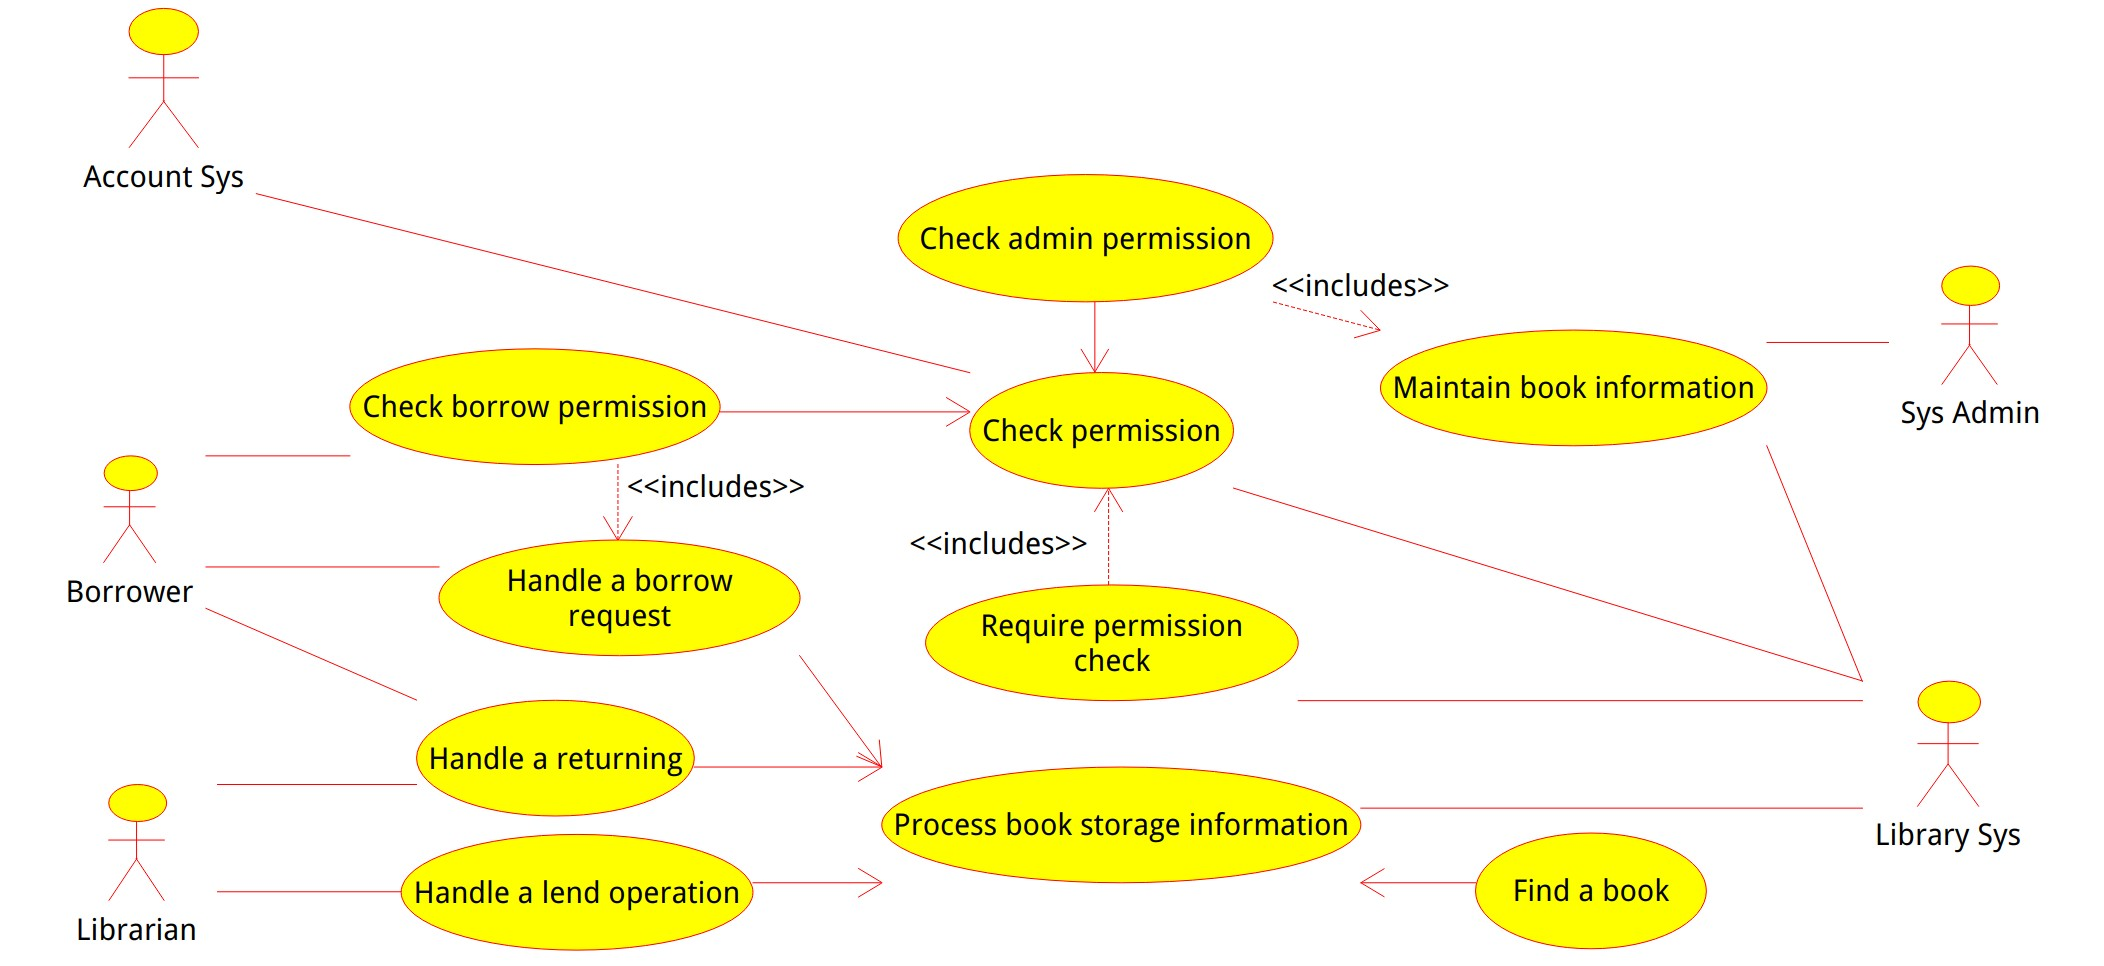
\includegraphics[scale=0.27]{pics/Library Use Case.jpg}
    \end{figure}
\end{document}